\documentclass[12pt, letterpaper, titlepage]{article}

\usepackage{amsmath}
\usepackage{booktabs}
\usepackage{amsthm}
\usepackage{graphicx}
\usepackage[margin=1in]{geometry}
\usepackage{hyperref}
\hypersetup{colorlinks = true, linkcolor = blue, citecolor=blue, urlcolor = blue}
\usepackage{natbib}
\usepackage{enumitem}
\usepackage{setspace}

\usepackage[pagewise]{lineno}
%\linenumbers*[1]
% %% patches to make lineno work better with amsmath
\newcommand*\patchAmsMathEnvironmentForLineno[1]{%
 \expandafter\let\csname old#1\expandafter\endcsname\csname #1\endcsname
 \expandafter\let\csname oldend#1\expandafter\endcsname\csname end#1\endcsname
 \renewenvironment{#1}%
 {\linenomath\csname old#1\endcsname}%
 {\csname oldend#1\endcsname\endlinenomath}}%
\newcommand*\patchBothAmsMathEnvironmentsForLineno[1]{%
 \patchAmsMathEnvironmentForLineno{#1}%
 \patchAmsMathEnvironmentForLineno{#1*}}%

\AtBeginDocument{%
 \patchBothAmsMathEnvironmentsForLineno{equation}%
 \patchBothAmsMathEnvironmentsForLineno{align}%
 \patchBothAmsMathEnvironmentsForLineno{flalign}%
 \patchBothAmsMathEnvironmentsForLineno{alignat}%
 \patchBothAmsMathEnvironmentsForLineno{gather}%
 \patchBothAmsMathEnvironmentsForLineno{multline}%
}

% control floats
\renewcommand\floatpagefraction{.9}
\renewcommand\topfraction{.9}
\renewcommand\bottomfraction{.9}
\renewcommand\textfraction{.1}
\setcounter{totalnumber}{50}
\setcounter{topnumber}{50}
\setcounter{bottomnumber}{50}

\newcommand{\jy}[1]{\textcolor{blue}{JY: #1}}
\newcommand{\eds}[1]{\textcolor{red}{EDS: (#1)}}


\title{On Misuses of the Kolmogorov--Smirnov Test for One-Sample Goodness-of-Fit}

\author{Anthony Zeimbekakis\\
%   \href{mailto:anthony.zeimbekakis@uconn.edu}
% {\nolinkurl{anthony.zeimbekakis@uconn.edu}}\\
  Elizabeth Schifano\\
  Jun Yan\\[1ex]
  Department of Statistics, University of Connecticut\\
}
\date{}

\begin{document}
\maketitle

\doublespace

\begin{abstract}
The Kolmogorov--Smirnov (KS) test is one of the most popular goodness-of-fit
tests for comparing a sample with a hypothesized continuous distribution.
Nevertheless, it has often been misused. The standard one-sample KS test applies
to independent, continuous data with a hypothesized distribution that is
completely specified. It is not uncommon, however, to see in the literature that
it was applied to dependent, discrete, or rounded data, with hypothesized
distributions containing estimated parameters. For example, it has been
``discovered'' multiple times that the test is too conservative when the 
hypothesized distribution has parameters that need to be estimated.
We demonstrate misuses of the one-sample KS test in
three scenarios through simulation studies:
1) the hypothesized distribution has unspecified parameters;
2) the data are serially dependent; and
3) a combination of the first two scenarios.
For each scenario, we provide remedies for practical applications.

\bigskip
\noindent{\sc Keywords}:
nonparametric bootstrap;
parametric bootstrap;
working dependence.
\end{abstract}

\section{Introduction}
\label{sec:intro}

The Kolmogorov-Smirnov (KS) test is one of the most popular goodness-of-fit
tests for comparing a sample with a hypothesized parametric distribution.
Let $X_1, ..., X_n$ be a random sample of size~$n$ from a continuous
distribution. The null hypothesis $H_0$ is that $X_i$'s follow distribution~$F$.
Let $F_n(t) = \sum_{i=1}^n I(X_i \le t) / n$ be the empirical cumulative
distribution function of the sample, where $I(\cdot)$ is the indicator
function. The KS test statistic is
\begin{equation}
  \label{eq:ks_standard}
  D_n = \sqrt{n} \sup_x | F_{n}(x) - F(x) |.
\end{equation}
The asymptotic distribution of $D_n$ under $H_0$ is independent of the
distribution~$F$. As $n \to \infty$, $D_n$ converges in distribution to
the supremum of standard Brownian bridge \citep{kolmogorov1933sulla}. For large
samples, the tests can be performed with a table \citep{smirnov1948table}.
Critical values for small samples ($n \le 35$) have also been given
\citep{massey1951kolmogorov}. The KS test is available in popular
statistical software packages, such as function \texttt{ks.test()} in R package
\textsf{stats} \citep{R, marsaglia2003evaluating}.


The standard one-sample KS test applies to independent data with a continuous
hypothesized distribution that is completely specified. In practice, however, it
has often been applied without realizing that one or more of these assumptions
do not hold. For example, \citet{noether1963note} showed the conservativeness of
the KS test when applied to discontinuous distributions. The null distribution
of the KS statistic is no longer distribution free. Computing the
exact and asymptotic distribution of $D_n$ is challenging. Fortunately, the null
distribution of the KS statistic for discontinuous distributions has been
efficiently addressed by \citet{dimitrova2020computing} with a
companion R package \textsf{KSgeneral}. Although a common misuse of KS test, the
issue with discontinuous data is not our focus.


When the hypothesized distribution~$F$ contains unspecified parameters, as is
the case in most goodness-of-fit test settings, the standard KS test is not
applicable. \citet{steinskog2007cautionary} ``discovers'' the change in power
when using fitted parameters and stresses caution in using the KS test in
such ways. In fact, using fitted parameters in place of the true parameters in
KS test has been long known to yield extremely conservative results
\citep[e.g.,][]{lilliefors1967kolmogorov}. This problem can be solved by
parametric bootstrap \citep{efron1985bootstrap, hall1991two}, where
bootstrap samples of the test statistics are constructed from samples
generated from the fitted hypothesized distribution. A nonparametric bootstrap
solution is not trivial because a nonparametric bootstrap sample of the
observed data has ties, which would not happen for continuous distributions.
\citet{babu2004goodness} derived the bias of the standard nonparametric 
bootstrap and
showed how to correct it. They further noted that both parametric and
nonparametric procedures lead to correct asymptotic levels.


The standard KS test does not apply to stationary yet dependent data either. The
distribution of the KS statistic would have a higher variance for positively
dependent data than that derived when the data are independent because of a
smaller effective sample size. For example, for testing normality,
\citet{durilleul1992lack} demonstrates that a naive application of
the KS statistic is too liberal for medium-to-high positive serial dependence,
and that for negative dependence, the behavior is asymmetrical. For remedies,
\citet{weiss1978modification} provides a procedure that is applicable 
specifically for data
modeled by the second-order auto-regressive (AR) process where the AR parameters
are known. \citet{lanzante2021testing} tests various strategies for dealing with
temporal
dependence and concludes that a test based on Monte-Carlo simulations performed
the best. When additionally the hypothesized distribution contains unknown
parameters, the standard KS test becomes even further
inapplicable. Practitioners, however, may have used the test without knowing its
limitations \citep[e.g.,][]{tuncer2019online}.


The contribution of this paper is a demonstration of misuses of the one-sample
KS test in three scenarios and their remedies in practice. The scenarios are
where:
1) the hypothesized distribution has unspecified parameters;
2) the data are serially dependent; and
3) a combination of the first two scenarios.
In each scenario, the misuse is performed and the impacts are shown. Then, a
remedy is detailed and performed alongside the misuse to show its positive
effects. In order to set up the demonstrations, simulated data are used
throughout. The remedies are also performed on various families of
distributions. An R implementation of the proposed methods will be available
after the paper is published.


The rest of the paper is organized as follows. Section~\ref{sec:fitted}
investigates the scenario where the hypothesized distribution has unspecified
parameters. Both parametric and nonparametric bootstrap are available to fix the
issue. Section~\ref{sec:dependence} investigates the scenario where the data of
the empirical distribution are serially dependent. A bootstrap procedure
employing copulas to account for dependence is proposed as a working solution.
Section~\ref{sec:fittedwithdependence}
explores the case where a combination of the first two scenarios occurs. The
copula procedure can be adjusted for the use of fitted parameters as a remedy.
Section~\ref{sec:conclusion} concludes with a discussion.

\section{Unspecified Parameters}
\label{sec:fitted}

The null hypothesis of a goodness-of-fit test is often a composite hypothesis
instead of a single hypothesis. That is, the hypothesized distribution is a
family of distributions with unspecified parameters instead of a specific member
in this family. Let $F_\theta$ be a family of distributions indexed by parameter
vector~$\theta$. The null hypothesis is
\[
  H_0: \text{the random sample $X_1, \ldots, X_n$
    comes from a distribution $F_\theta$ for some $\theta$.}
\]
Since $\theta$ is unknown, one would naturally estimate $\theta$ by
$\hat\theta_n$ from, for example, maximum likelihood or methods of moments. The
KS statistic would then be computed as
\begin{equation}
  \label{eq:ks_fitted}
  D_n = \sqrt{n} \sup_x | F_n(x) - F_{\hat\theta_n}(x) |.
\end{equation}
An overly large $D_n$ still indicates evidence to reject~$H_0$. To get the
p-value of the observed $D_n$, however, note that the null distribution is not
the same as that in the standard
case~\eqref{eq:ks_standard}. If the same null distribution were used, one would
be testing a different~$H_0$ that the random sample comes from the specific
member distribution~$F_{\hat\theta}$ instead of the family~$F_\theta$.


The consequence of using the wrong null distribution for the KS statistic $D_n$
in~\eqref{eq:ks_fitted} can be illustrated through a simple simulation study. A
random sample $X_1, \ldots, X_n$ was generated from the standard normal
distribution with sample size $n = 100$. The sample mean and sample standard
deviation were used as $\hat\theta_n$. The p-value of the test
statistic~$D_n$ in~\eqref{eq:ks_fitted} was obtained by naively calling the
\texttt{ks.test()} function in~R with the fitted normal distribution as the
hypothesized distribution. That is, the hypothesized distribution was
$N(\bar X, s^2)$ where $\bar X$ is the sample mean and $s^2$ is the sample
variance. This experiment was repeated 1000 times and the histogram of the
1000 p-values are displayed in Figure~\ref{fig:hist_fitted}. If the test were
valid, the p-values would be uniformly distributed in the unit
interval. Clearly, the pattern of the 1000 p-values are very different from what
one would expect to see from 1000 draws from the standard uniform
distribution.


To fix the problem, parametric bootstrap can be used to approximate the null
distribution of the test statistic~$D_n$:
\begin{enumerate}
\item
  Draw a random sample $X_1^*,...,X_n^*$ from the fitted distribution
  $F_{\hat\theta_n}$
\item
  Fit $F_\theta$ to $X_1^*,...,X_n^*$ and obtain estimate 
	$\hat\theta_n^*$ of $\theta$.
\item
  Obtain the empirical distribution function $F_n^*$ of
  $X_1^*, \ldots,  X_n^*$.
\item
  Calculate bootstrap KS statistic
  \[
    D_n^* = \sqrt{n} \sup_x | F_n^* (x)- F_{\hat\theta_n^*}(x) |.
  \]
\item
  Repeat the previous steps a large number~$B$ times and use the empirical
  distribution of $D_n^*$ to approximate the null distribution of the observed
  statistic.
\end{enumerate}
The p-value of $D_n$ is approximated by the proportion of the $D_n^*$ 
statistics that are
greater than or equal to~$D_n$.


Nonparametric bootstrap can also be used to approximate the null distribution
of the test statistic with the bias correction from \citet{babu2004goodness}:
\begin{enumerate}
\item
  Draw a random sample $X_1^*,...,X_n^*$ from the empirical distribution $F_n$
  with replacement
\item
  Fit $F_\theta$ to $X_1^*,...,X_n^*$ and obtain estimate 
	$\hat\theta_n^*$ of $\theta$.
\item
  Obtain the empirical distribution function $F_n^*$ of
  $X_1^*, \ldots,  X_n^*$. \eds{verify edit}
\item
  Calculate bootstrap KS statistic
  \[
    D_n^* = \sup_x | \sqrt{n}\left(F_n^* (x)- F_{\hat\theta_n^*}(x)\right) - B_n(x) |.
  \]
  where $B_{n}(x) = \sqrt{n}(F_{n}(x) - F_{\hat\theta_n}(x))$ is the known
  bias term \citep{babu2004goodness}.
\item
  Repeat the previous steps a large number $B$ times and use the empirical
  distribution of $D_n^*$ to approximate the null distribution of the observed
  statistic. 
\end{enumerate}
The p-value of $D_n$ is, again, approximated by the proportion of the $D_n^*$
statistics that are greater than or equal to~$D_n$. Note that the step~1 and
step~4 are different from the parametric bootstrap version.


\begin{figure}[tbp]
  \centering
  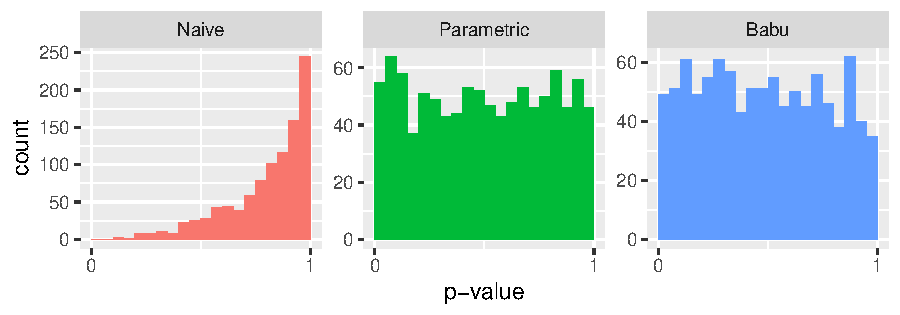
\includegraphics[width=\textwidth]{hist_fitted}
  \caption{Histograms of p-values for the KS test with unspecified parameters in
    the hypothesized distribution based on 1000 replicates of sample size
    $n = 100$. Naive (left): KS test with KS statistic calculated based on fitted
    parameters. Parametric bootstrap (center): KS test with parametric
    bootstrap. Nonparametric bootstrap (right): KS test with nonparametric
    bootstrap using the bias correction from \citet{babu2004goodness}.
    \eds{perhaps use density hist vs
	freq. hist (here and elsewhere)?}}
  \label{fig:hist_fitted}
\end{figure}

\jy{Anthony, could you label the panels as ``Parametric bootstrap'' and
  ``Nonparametric bootstrap'' for the center and right panels?}

\jy{Simulation study: let's use two distributions:
  $N(8, 8)$ and $\Gamma(8, 1)$. These two distributions have the same means and
  variances. So we could use them to study powers of the tests too.}

In the same simulation study, p-values were obtained for the 1000 replicates
with both the parametric and nonparametric bootstrap procedures. The center and
right panels of Figure~\ref{fig:hist_fitted} display the histograms of the 1000
p-values from the parametric and nonparametric bootstrap procedures,
respectively. This time, both samples of p-values appear to come from
standard uniform distributions.

\section{Serially Dependent Data}
\label{sec:dependence}

Here we consider the situation where the observed data $X_1, \ldots, X_n$ are
not independent but serially dependent, and the hypothesized distribution $F$
contains no unknown parameters. That is,
\[
H_0: \text{$X_i$'s have marginal distribution $F$.}
\]
The KS statistic $D_n$ in~\eqref{eq:ks_standard}
is still a good measure of deviation from the null hypothesis. Nonetheless, the
null distribution of $F_n$ changes when there is serial dependence.
When the serial dependence is
positive, the effective sample size is less than~$n$. The test statistic
would be stochastically greater than that obtained from independent data, 
resulting in a test that is too liberal (i.e., the null hypothesis is rejected
more often than it should). The reasoning is similar when the serial dependence 
is negative, in which case, the test is conservative.

\jy{For the same two marginal distributions $N(8, 8)$ and $\Gamma(8, 1)$, let's
  generate data from dependence structures of AR(1) with two coefficients
  $\psi \in \{ -0. 5, 0.5\}$.}

The invalidity of the standard statistic for serially dependent data can be
illustrated by a simple simulation study. Consider a first-order autoregressive
or AR(1) model with marginal standard normal distribution. For each AR
coefficient $\psi \in \{-0.3, 0.2, 0.1, 0, 0.1, 0.2, 0.3\}$, we generated 1000
series of length 100. For each series, we applied the KS statistic
in~\eqref{eq:ks_standard} to test $H_0$ that the $X_i$'s follow $N(0, 1)$
marginally. The histograms of the p-values from $1000$ replicates for all the
$\psi$ values are displayed in Figure~\ref{fig:hist_correlation}. When
$\phi \ne 0$, the histograms do not look likely to be generated from a standard
uniform distribution. Positive $\psi$ values led to p-values with a distribution
function higher than the standard uniform distribution function and, hence,
conservative tests. Negative $\psi$ values led to p-values with a distribution
function lower than the standard uniform distribution and, hence, liberal
tests. The larger the magnitude of
$\psi$, the bigger the deviation from the desired level.

\begin{figure}[tbp]
  \centering
  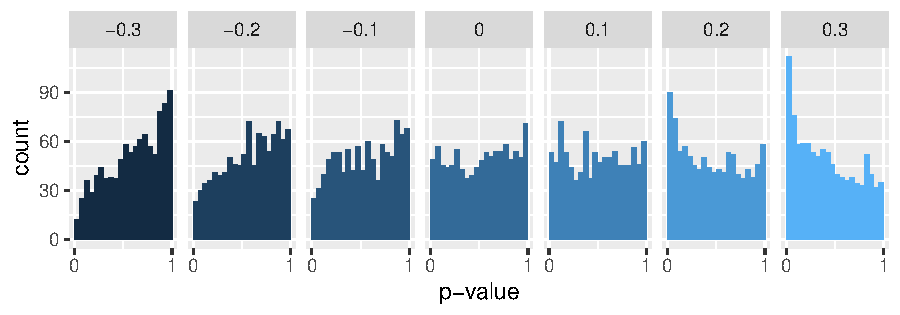
\includegraphics[width=\textwidth]{hist_correlation}
  \caption{Histograms of p-values for the KS test applied to data generated from
    AR(1) processes with AR coefficients
    $\psi \in \{-0.3, -0.2, -0.1, 0, 0.1, 0.2, 0.3\}$
    based on 1000 replicates of sample size $n = 100$.}
  \label{fig:hist_correlation}
\end{figure}


A complete remedy for KS tests with serially dependent data is
challenging. The null distribution depends on the structure of the serial
dependence, which can be arbitrary in practice. A parametric bootstrap procedure
would need to specify a model for the dependence, whereas the primary interest
is to test the marginal distribution of the stationary series. A block
nonparametric bootstrap for stationary data \citep{kunsch1989jackknife} is
tempting, but the counterpart of a bias correction as in
\citet{babu2004goodness} is not available yet. Is there any approach that does
not require full specification of the dependence of the stationary process,
but still gives reasonably satisfactory correction to the size of the KS test in
certain applications?


We propose a semiparametric bootstrap procedure that assumes a working serial
dependence structure which does not need to be correctly specified. The working
serial dependence is introduced through copulas with the hope to approximate the
true serial dependence as allowed by the working copulas. A copula is a
multivariate distribution with standard uniform marginal distributions, which
completely characterizes the dependence structure of a multivariate
distribution \citep{hofert2018elements}. It separates the dependence structure
of a multivariate distribution from its marginal distributions. The normal copula
is the copula determined by the multivariate normal distribution. We propose to
use a normal working copula to approximate the serial
dependence of the observations.


The parameters of the working normal copula are
estimated from fitting an auto-regressive moving average (ARMA) model to the
observed data transformed to the standard normal scale. In particular, let
$Z_i = \Phi^{-1}\{ F(X_i)\}$, $i = 1, \ldots, n$, where $\Phi$ is the distribution
function of the standard normal. Then we fit an ARMA$(p, q)$ model to
$Z_1, \ldots, Z_n$ with AR order $p$ and MA order $q$ selected by the Akaike
Information Criterion (AIC). This can be done with, for example, function
\texttt{auto.arima()} from  R package \texttt{forecast}
\citep{hyndman2008automatic}. Since it is known that the mean of $Z_i$'s is
zero, it is necessary to set the intercept of the ARMA model as zero in the
fitting process. This restriction turned out to be critical in our
investigation; having the intercept estimated does not lead to desired p-value
distributions in the following bootstrap process.
The selected ARMA$(p, q)$ model with fitted
parameters will be used as the working model to generate bootstrap samples with
serial dependence mimicking that in the observed data. The unconditional
variance $\sigma^2$ of the ARMA model with unit innovation variance can be
obtained with function
\texttt{tacvfARMA()} from R package \texttt{ltsa} \citep{mcleod2007algorithms}.


The semiparametric bootstrap procedure is as follows.
\begin{enumerate}
\item
  Generate $Z_1^*, \ldots, Z_n^*$ from the fitted ARMA$(p, q)$ process with
  innovation \eds{? inverse?} variance $1 / \sigma^2$ such that the $Z_i$'s are
	marginally \jy{yes, it means the innovation series of an ARMA process.}
  standard normal variables.
\item
  Form a bootstrap sample $X_i^* = F^{-1} [\Phi(Z_i^*)]$,  $i = 1, \ldots, n$.
\item
  Obtain the empirical distribution function $F_n^*$ of the bootstrap sample
  $X_1^*, \ldots, X_n^*$.
\item
  Calculate bootstrap KS statistic
  \[
    D_n^* = \sup_x \lvert F_n^* (x)- F(x) \rvert.
  \]
\item
  Repeat the previous steps a large number $B$ times and use the empirical
  distribution of the $B$ test statistics to approximate
  the null distribution of the observed statistic.
\end{enumerate}
The p-value of $D_n$ is, again, approximated by the proportion of the $D_n^*$
statistics that are greater than or equal to~$D_n$. 


This process is semiparametric because the marginal distribution is
parametrically specified while the dependence structure of the stationary series
is only approximated by that of an ARMA process with normal distributions.
The closer the approximation is to the truth, the better
performance of the size of the KS test. The normal copula of the working ARMA
process provides a wide class of dependence structures.
If the true dependence indeed has an ARMA structure, this method is exact. When
the true dependence is not covered by the ARMA model, the working model may 
still give a reasonable approximation that can
be useful for practical purposes. 


\jy{Here we work on the same marginal distributions $N(8, 8)$ and $\Gamma(8, 1)$
  with different dependence structures:
  ARMA(1, 1); MA(2); AR(2)
  }
Continuing with the simulation study, 
Throughout the simulation we assume a working AR(1) dependence structure
regardless of the true dependence. This is demonstrated with different dependence
structures in Figure~\ref{fig:hist_ma1_arma_ar2_D}.

\begin{figure}[tbp]
  \centering
  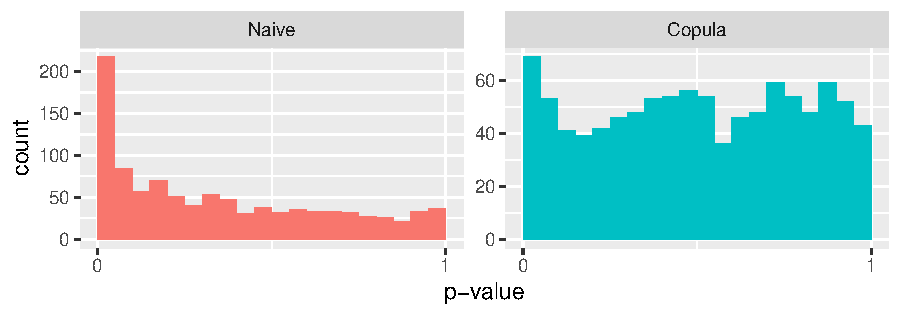
\includegraphics[width=\textwidth]{hist_ar1_D}
  \caption{The Naive plot (left) is the histogram of p-values from the
  standard KS test. The Copula plot (right) is the histogram of p-values from
  implementing the parametric \eds{semiparametric?} bootstrap with copulas for
	dependence. In each case,
  $1000$ replicate tests were performed with the data generated from an AR(1)
  process of the standard normal distribution with $\psi = .5$. The sample size
  is $n = 100$ and $B = 1000$ bootstrap samples are obtained for each test.}
  \label{fig:hist_ar1_D}
\end{figure}

Figure~\ref{fig:hist_ar1_D} displays the results of the copula remedy for
dependent data. The data is generated from the standard normal distribution with
an AR(1) dependence structure where $\psi = .5$. The copula used is to model
dependence is the normal copula. The distribution of p-values is again expected
to be $U(0, 1)$ for a valid test. The Naive plot is clearly not uniform and
reinforces the results shown in Figure~\ref{fig:hist_correlation}. The Copula
plot, which implements the aforementioned procedure to correct for dependence
in the data, appears to be uniform and restores the size of the KS test.


\begin{figure}[tbp]
  \centering
  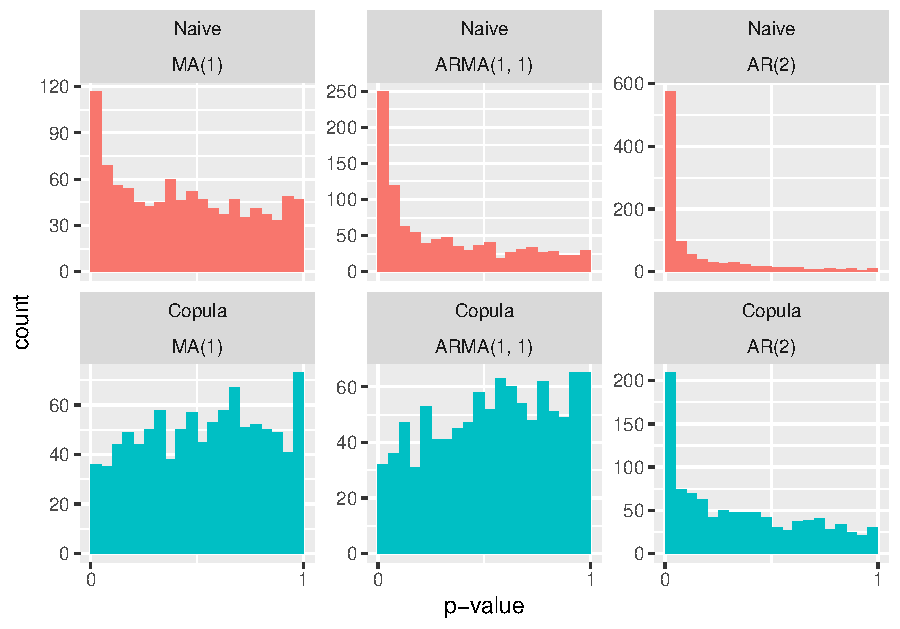
\includegraphics[width=\textwidth]{hist_ma1_arma_ar2_D}
  \caption{The Naive plots are the histograms of p-values from the standard KS
  test. The Copula plots are the histograms of p-values from parametric
  bootstrap with copulas for dependence. The data is generated from an MA(1)
  process (left) with $\theta = .5$, ARMA(1, 1) process (middle) with $\psi =
  .5$ and $\theta = .3$, and AR(2) process (right) with $\psi = (.5, .3)$ of the
  standard normal distribution. In each case, $1000$ replicate tests were
  performed with sample size $n = 100$ and $B = 1000$ bootstrap samples.}
  \label{fig:hist_ma1_arma_ar2_D}
\end{figure}

\jy{to be rewritten when the figures are generated.}
\jy{I suggest that we keep using gamma as the marginal distribution
  throughout. Elizabeth, let's finalize the settings next time we meet. I've
  implemented a concise version of the test.}

The procedure detailed in this section can also provide a reasonable
approximation in cases where the true dependence structure is not far from
AR(1). Figure~\ref{fig:hist_ma1_arma_ar2_D} shows the distribution of p-values
for dependence structures MA(1), ARMA(1, 1), and AR(2). As expected,
naively performing the KS test without correcting for dependence provides plots
of p-values that deviate from the uniform distribution. In the case of MA(1)
and ARMA(1, 1), the true dependence structure is close enough to our
assumption of AR(1) that the bootstrap procedure provides a reasonable
approximation. However, the AR(2) copula plot shows the limitation of this
technique as no AR(1) process can approximate an AR(2) process unless the
second-order coefficient is close to zero.

\begin{figure}[tbp]
  \centering
  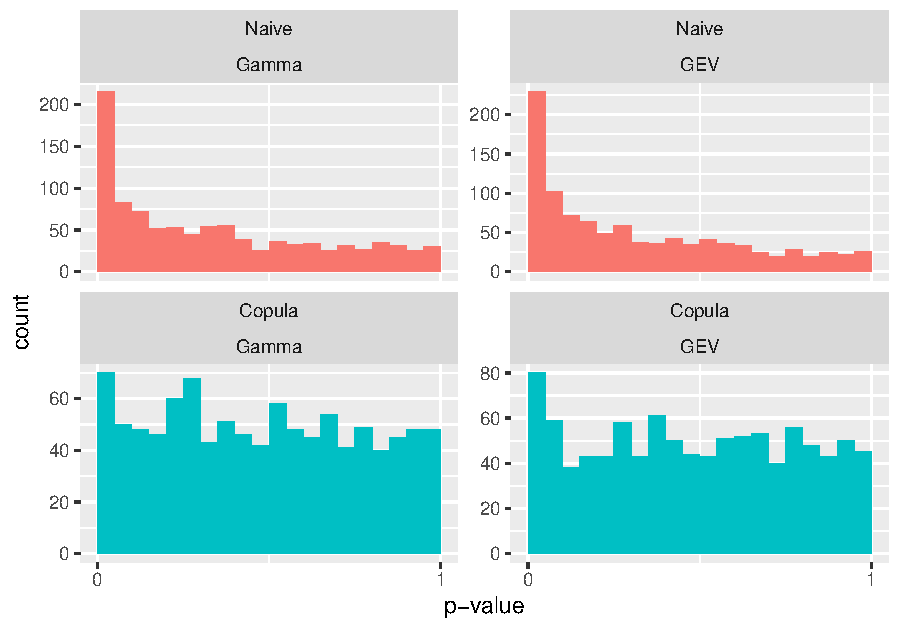
\includegraphics[width=\textwidth]{hist_gamma_gev_D}
  \caption{The Naive plots are the histograms of p-values from the standard KS
  test. The Copula plots are the histograms of p-values from parametric
  bootstrap with copulas for dependence. The data is generated from $Gamma(3,
  1)$ (left) and $GEV(0, .2, 1)$ (right) with a correlation coefficient of $r =
  0.5$. In each case, $1000$ replicate tests were performed with sample size $n
  = 100$ and $B = 1000$ bootstrap samples.}
  \label{fig:hist_gamma_gev_D}
\end{figure}

To further demonstrate the effectiveness of the procedure, we perform similar
simulations on other families of distributions.
Figure~\ref{fig:hist_gamma_gev_D} displays the results of tests using dependent
data generated from the gamma and the generalized extreme value distributions.
The procedure corrects the distribution of p-values for both distributions and
is shown to be applicable regardless of the family of distribution tested.


\section{Unspecified Parameters and Serially Dependent Data}
\label{sec:fittedwithdependence}

When the observed sample $X_1, \ldots, X_n$ is no longer a random sample but
a serially dependent stationary series, we may still be interested in testing
whether marginally each $X_i$ follows hypothesized distribution with unknown
parameters. That is, the null hypothesis is
\[
H_0: \text{$X_i$'s have marginal distribution $F_\theta$ for some $\theta$}.
\]
The testing statistic $D_n$ in Equation~\eqref{eq:ks_fitted} still measures the
deviation from $H_0$, but its null distribution depends on the serial
dependence. The bootstrap procedure in the last section can be adapted to handle
this situation.


Specifically, let $\hat\theta_n$ be the marginally fitted parameters, and
$Z_i = \Phi^{-1} \{F_{\hat\theta_n}(X_i)\}$, $i = 1, \ldots, n$ be a
transformation of the observed data onto the standard normal scale using the
fitted parameters $\hat\theta_n$. We then fit an ARMA model with orders
selected by the AIC using function \texttt{auto.arima()} from R package
\texttt{forecase}. This ARMA model will be used as the working model to
introduce serial dependence in the bootstrap samples. Similarly, we obtain the
unconditional variance $\sigma^2$ of the ARMA process with unit innovation
variance. Our semiparametric bootstrap procedure is as follows

\begin{enumerate}
\item
  Generate $Z_1^*, \ldots, Z_n^*$ from the working ARMA$(p, q)$ model with
  innovation variance $1 / \sigma^2$ such that the $Z_i$'s are marginally
  standard normal variables.
\item
  Form a bootstrap sample
  $X_i^* = F_{\hat\theta_n}^{-1} [\Phi(Z_i^*)]$, $i = 1, \ldots, n$.
\item
  Fir $F_\theta$ to $X_1^*, \ldots, X_n^*$ to obtain estimate $\hat\theta_n^*$
  of $\theta$.
\item
  Obtain the empirical distribution function $F_n^*$ of the bootstrap sample
  $X_1^*, \ldots, X_n^*$.
\item
  Calculate bootstrap KS statistic
  \[
    D_n^* = \sup_x \lvert F_n^* (x) - F_{\hat\theta_n}^* (x) \rvert.
  \]
\item
  Repeat the previous steps a large number $B$ times and use the empirical
  distribution of the $B$ test statistics to approximate
  the null distribution of the observed statistic.
\end{enumerate}
The p-value of $D_n$ is approximated by the proportion of the $D_n^*$
statistics that are greater than or equal to~$D_n$. Compared to the algorithm in
the last section, here we use $F_{\hat\theta_n}$ and $F_{\hat\theta_n}^*$ in
place of the known~$F$.


\jy{For the simulation study, repeat the study at the end of the last section.}  

\begin{figure}[tbp]
  \centering
  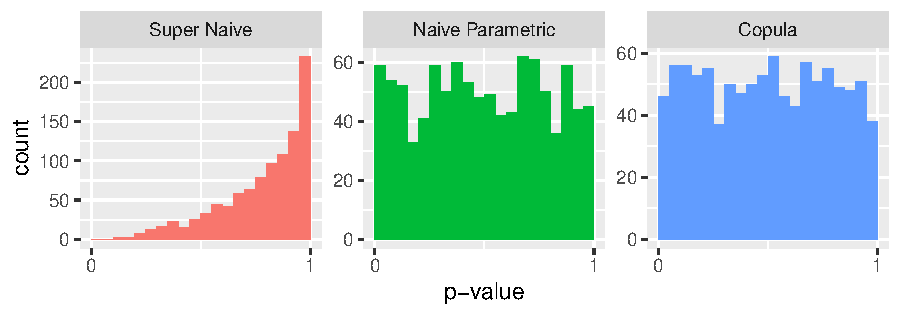
\includegraphics[width=\textwidth]{hist_ar1_FD}
  \caption{The Super Naive plot (left) is the histogram of p-values from the
  standard KS test with fitted parameters. The Naive Parametric plot (middle) is
  the histogram of p-values from implementing parametric bootstrap. The Copula
  plot is the histogram of p-values from implementing parametric bootstrap with
  copulas for dependence and correcting for fitted parameters. In each case,
  $1000$ replicate tests were performed with the data generated from an AR(1)
  process of the standard normal distribution with $\psi = .5$. The sample size
  is $n = 100$ and $B = 1000$ bootstrap samples are obtained for each test.}
  \label{fig:hist_ar1_FD}
\end{figure}


Figure~\ref{fig:hist_ar1_FD} shows the results of our simulation on data
simulated from an AR(1) process. As should be expected, naively fitting
parameters while providing no adjustment for dependent data invalidates the KS
test. As well, only using the parametric bootstrap remedy for fitted parameters
from Section~\ref{sec:fitted} seems to provide weaker results than the
copula remedy presented above. The results show that copula remedy generates
uniform p-values and restores the size of the KS test.

\begin{figure}[tbp]
  \centering
  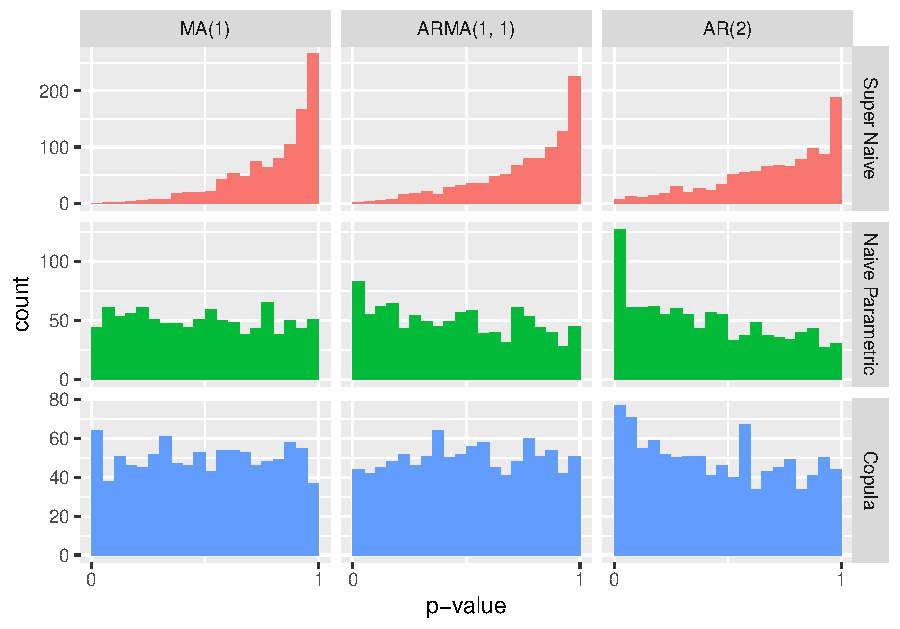
\includegraphics[width=\textwidth]{hist_ma1_arma_ar2_FD}
  \caption{The Super Naive plots (left) are the histograms of p-values from the
  standard KS test with fitted parameters. The Naive Parametric plots (middle)
  are the histograms of p-values from implementing parametric bootstrap. The
  Copula plots (bottom) are the histograms of p-values from implementing
  parametric bootstrap with copulas for dependence and correcting for fitted
  parameters. The data is generated from an MA(1) process (left) with
  $\theta = .5$, ARMA(1, 1) process (middle) with $\psi = .5$ and $\theta = .3$,
  and AR(2) process (right) with $\psi = (.5, .3)$ of the standard normal
  distribution. In each case, $1000$ replicate tests were performed with sample
  size $n = 100$ and $B = 1000$ bootstrap samples.}
  \label{fig:hist_ma1_arma_ar2_FD}
\end{figure}

Similar to Section~\ref{sec:dependence}, the copula approach is not a complete
solution. Regardless of the true dependence in the data we assume an AR(1)
dependence structure by taking the lag-1 sample auto-spearman rho. However, we
can show that as long as the AR(1) assumption is a close approximation, the
correction still provides a reasonable approximation that can be useful for
practical purposes. Figure~\ref{fig:hist_ma1_arma_ar2_FD} shows the results of the
procedure performed on data generated with dependence structures of  MA(1),
ARMA(1, 1), and AR(2). Naively fitting parameters and not adjusting for
dependence clearly deviates from a uniform distribution of p-values. Parametric
bootstrap provides some correction but does not account for dependence, so
therefore the results of the copula remedy are more accurate and favorable.
In the case of MA(1) and ARMA(1, 1), the true dependence appears close enough
to our assumption of AR(1) that the results are reasonable. AR(2) however
appears to be just far enough from our assumption, showing a limitation of the
procedure.

\begin{figure}[tbp]
  \centering
  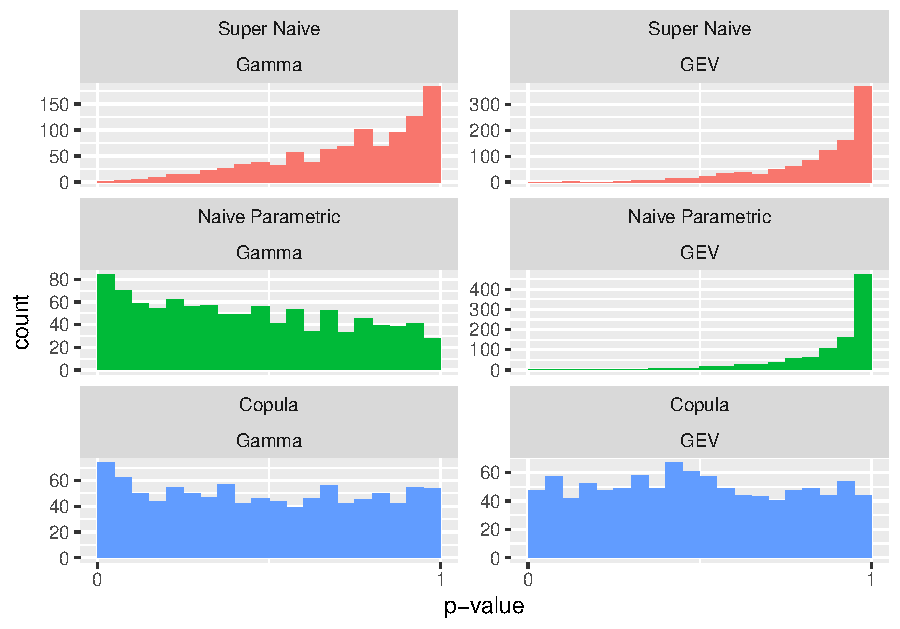
\includegraphics[width=\textwidth]{hist_gamma_gev_FD}
  \caption{The Super Naive plots (left) are the histograms of p-values from the
  standard KS test with fitted parameters. The Naive Parametric plots (middle)
  are the histograms of p-values from implementing parametric bootstrap. The
  Copula plots are the histograms of p-values from implementing parametric
  bootstrap with copulas for dependence and correcting for fitted parameters.
  The data is generated from $Gamma(3, 1)$ (left) and $GEV(0, .2, 1)$ (right)
  with a correlation coefficient of $r = 0.5$. In each case, $1000$ replicate
  tests were performed with sample size $n = 100$ and $B = 1000$ bootstrap
  samples.}
  \label{fig:hist_gamma_gev_FD}
\end{figure}

It is also possible to apply our procedure to other families of distributions.
The data in Figure~\ref{fig:hist_gamma_gev_FD} is generated from the gamma and
generalized extreme value distributions. The results are favorable and show that
the procedure outlined as a remedy for fitted parameters and spatially dependent
can be adapted for various families of distributions.


\section{Conclusion}
\label{sec:conclusion}

The KS test has base assumptions that the hypothesized distribution is
completely specified and the data is independent. When these assumptions are
violated, the test is no longer accurate and remedies must be performed. In the
case of fitted parameters, parametric and non-parametric bootstrap can restore
the size of the test. A bias correction is required if the non-parametric form
is used \citep{babu2004goodness}. In the case of \eds{serially} dependent data, a procedure
using bootstrap
with copulas to model dependency shows positive results. When both assumptions
are violated, i.e., where the data has \eds{serial} dependence and parameters
must
be fitted, an adjusted copula procedure also shows positive results. The tests
appear effective for a variety of families of distributions. The copula remedy
is not a complete solution and has limitations. Regardless of the true
dependence, we assume an AR(1) dependence structure. Therefore, if the AR(1)
dependence structure is a close approximation of the truth, the approach can work.
However, in cases such as AR(2), if the approximation is too far from the true
dependence structure the approach does not completely remedy the issue. As well,
tests were only performed with the normal copula. It is possible that other
copulas could provide stronger results based on the true dependence of the data.

\bibliographystyle{asa}
\bibliography{citations}


\end{document}
%%% LocalWords: 
%%% Local Variables:
%%% mode: latex
%%% TeX-master: t
%%% ispell-personal-dictionary: ".aspell.en.pws"
%%% fill-column: 80
%%% eval: (auto-fill-mode 1)
%%% End:
